\chapter{Junction Breakdown and Heterojunctions}
\label{ch:breakdown-heterojunctions}

Large reverse bias can activate interband tunneling or avalanche multiplication.
Both processes produce a rapid current increase, but their microscopic origins
and doping dependence differ.  A junction between different semiconductors adds
band offsets and unequal material parameters to the same Poisson and charge-
neutrality structure.  This chapter follows the breakdown and heterojunction
sequence of Sze and Lee \cite[Chap.~3, Secs.~3.6--3.7]{szeLee2012}.

\section{Tunneling breakdown}

In a heavily doped reverse-biased junction, depletion width is small and the
field can be large at modest voltage.  Occupied valence-band states on the
p-side can then tunnel directly into empty conduction-band states on the
n-side.  This band-to-band process is often called Zener breakdown.  A
WKB description contains the characteristic field dependence
\begin{equation}
 G_{\mathrm{BTBT}}\propto E^2
 \exp\left[-\frac{B_{\mathrm{BTBT}}}{|E|}\right],
 \label{eq:band-to-band-tunneling-generation}
\end{equation}
where $B_{\mathrm{BTBT}}$ depends on band gap and tunneling effective mass.
Heavy doping favors tunneling because it narrows the barrier and raises the
peak field.

\section{Avalanche multiplication}

An energetic electron or hole can create an electron--hole pair by impact
ionization.  The generated carriers accelerate and may create further pairs.
The local coefficients introduced in \cref{eq:impact-ionization-coefficient}
are
\begin{equation}
 \alpha_n(E)=A_n e^{-B_n/|E|},
 \qquad
 \alpha_p(E)=A_p e^{-B_p/|E|},
 \label{eq:junction-ionization-coefficients}
\end{equation}
with units $\mathrm{m^{-1}}$.  They are mean pair-production events per unit
carrier path length.

For equal coefficients, $\alpha_n=\alpha_p=\alpha$, multiplication diverges
when
\begin{equation}
 \boxed{\int_0^W\alpha[E(x)]\,\dd x=1.}
 \label{eq:equal-alpha-breakdown-condition}
\end{equation}
Unequal coefficients require the coupled electron and hole multiplication
equations and depend on the location of carrier injection.  The equal-$\alpha$
criterion remains a transparent numerical model of field-distributed feedback.

For a one-sided abrupt junction,
\begin{equation}
 W=\sqrt{\frac{2\varepsilon_s(V_{\mathrm{bi}}+V_R)}{qN_B}},
 \qquad
 |E(x)|=E_m\left(1-\frac{x}{W}\right),
 \qquad
 E_m=\frac{qN_BW}{\varepsilon_s},
 \label{eq:avalanche-triangular-field}
\end{equation}
where $N_B$ is the lightly doped background.  Numerical quadrature of
\cref{eq:equal-alpha-breakdown-condition} followed by scalar root finding gives
the avalanche voltage.  Increasing $N_B$ raises field for a given voltage but
reduces width; the exponential field dependence usually dominates and lowers
the breakdown voltage.

\begin{figure}[htbp]
 \centering
 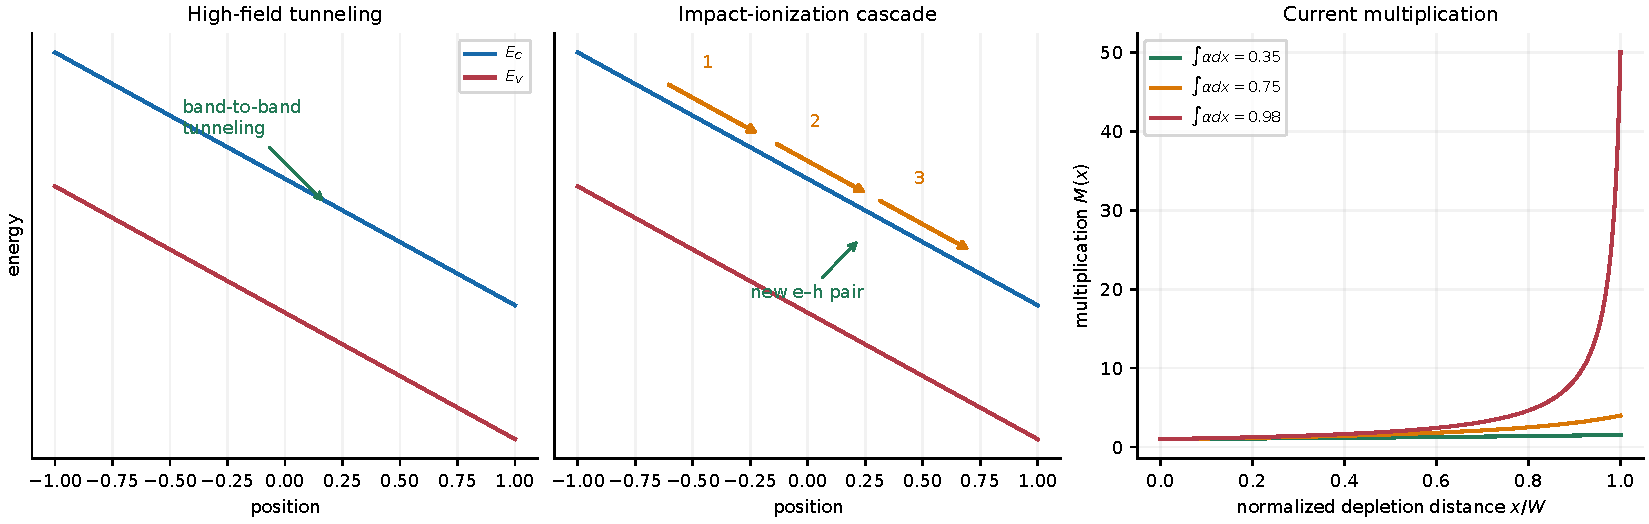
\includegraphics[width=\textwidth]{figures/junction-atlas-breakdown-mechanisms.pdf}
 \caption{Original band-diagram schematics of band-to-band tunneling and an
 impact-ionization cascade, together with spatial current multiplication.  The
 panels cover the physical content of Figs.~22--23 in Sze--Lee Chapter~3
 \cite[Secs.~3.6.1--3.6.2]{szeLee2012}.\figurenotebookmark}
 \label{fig:junction-atlas-breakdown-mechanisms}
\end{figure}
\figurenotebooktext{figures/20_breakdown-heterojunctions/fig_20_01.ipynb}

\begin{figure}[htbp]
 \centering
 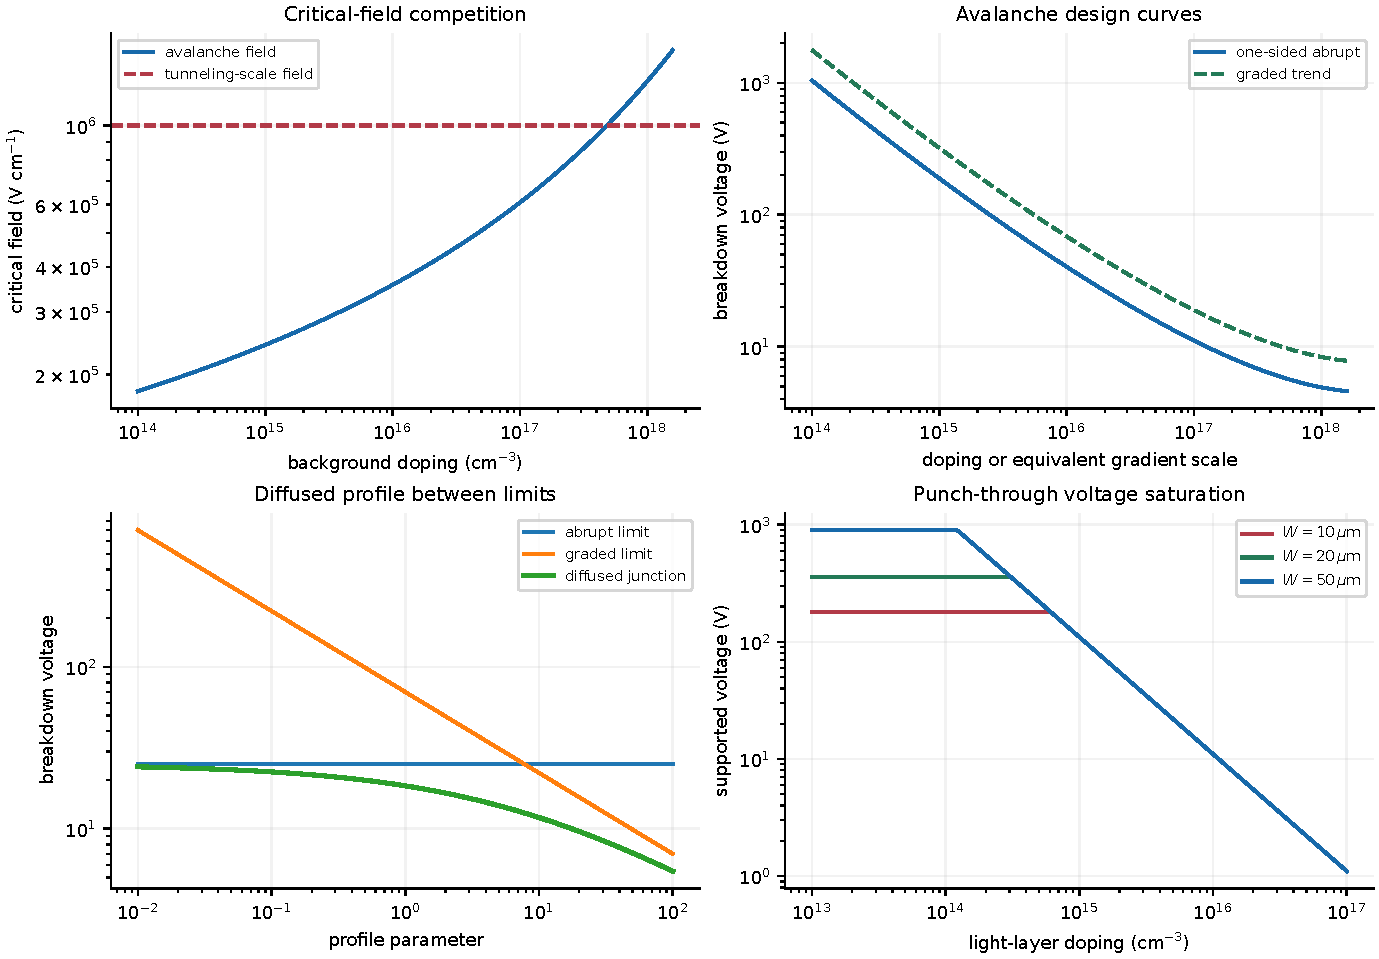
\includegraphics[width=\textwidth]{figures/junction-atlas-breakdown-design.pdf}
 \caption{Equation-generated critical-field competition, abrupt and graded
 avalanche trends, a diffused profile between limiting cases, and
 punch-through voltage saturation.  These panels cover the design comparisons
 of Figs.~24--27 in Sze--Lee Chapter~3 \cite[Sec.~3.6.2]{szeLee2012}.\figurenotebookmark}
 \label{fig:junction-atlas-breakdown-design}
\end{figure}
\figurenotebooktext{figures/20_breakdown-heterojunctions/fig_20_01.ipynb}

\section{Premature breakdown and geometry}

Planar processing bends junctions near mask edges.  Electric-field lines crowd
at cylindrical or spherical curvature, so the local peak field exceeds the
one-dimensional value.  Surface charge and defects can further enhance local
field.  A real device may therefore break down below the ideal plane-junction
prediction.  Guard rings, field plates, and graded termination regions spread
the field and increase usable voltage \cite[Sec.~3.6.3]{szeLee2012}.

Breakdown itself need not be destructive if current and temperature are
limited.  Uncontrolled power $P=IV$ can cause thermal runaway, filamentation,
or permanent damage.

\begin{figure}[htbp]
 \centering
 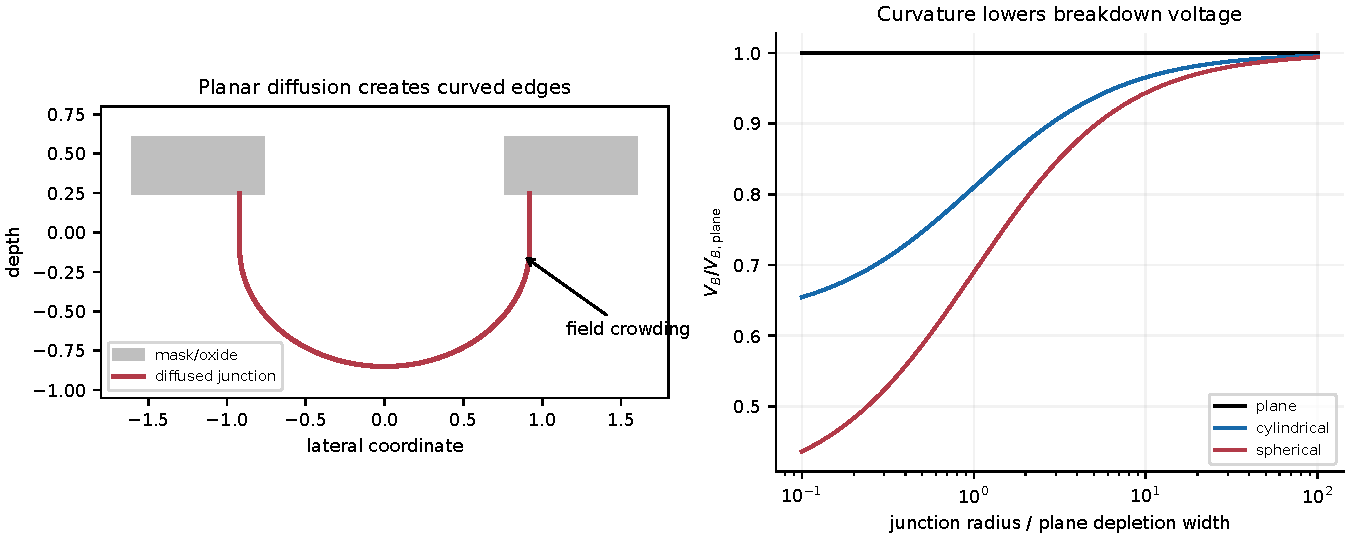
\includegraphics[width=0.92\textwidth]{figures/junction-atlas-curvature.pdf}
 \caption{Original planar-diffusion edge geometry and the reduction of
 breakdown voltage by cylindrical and spherical curvature.  The panels cover
 the subjects of Figs.~28--29 in Sze--Lee Chapter~3
 \cite[Sec.~3.6.3]{szeLee2012}.\figurenotebookmark}
 \label{fig:junction-atlas-curvature}
\end{figure}
\figurenotebooktext{figures/20_breakdown-heterojunctions/fig_20_01.ipynb}

\section{Heterojunction band offsets}

\begin{definition}{Heterojunction}{heterojunction}
A heterojunction is an interface between semiconductors with different band
structures.  A homojunction joins differently doped regions of the same
semiconductor.  An isotype heterojunction joins the same conductivity type;
an anisotype heterojunction joins opposite types.
\end{definition}

Let material $j$ have electron affinity $\chi_j$ and band gap $E_{gj}$, both in
electron-volts.  The ideal electron-affinity rule aligns vacuum levels before
contact and predicts
\begin{align}
 \Delta E_C&=E_{C2}-E_{C1}=\chi_1-\chi_2,
 \label{eq:anderson-conduction-offset}\\
 \Delta E_V&=E_{V2}-E_{V1}
 =\chi_1+E_{g1}-\chi_2-E_{g2}.
 \label{eq:anderson-valence-offset}
\end{align}
These definitions satisfy
$\Delta E_C-\Delta E_V=E_{g2}-E_{g1}$.  The conduction offset filters electrons;
the valence offset filters holes.  Interface dipoles, chemical bonding, strain,
and polarization can shift real offsets away from the electron-affinity rule.

At equilibrium, the Fermi level remains constant across the heterojunction.
Poisson's equation applies on both sides, but permittivity and doping differ.
For depletion charges $Q_1=-Q_2=Q$, the potential drops are
\begin{equation}
 |\psi_1|=\frac{Q^2}{2q\varepsilon_1N_1},
 \qquad
 |\psi_2|=\frac{Q^2}{2q\varepsilon_2N_2}.
 \label{eq:heterojunction-potential-partition}
\end{equation}
Thus voltage partition depends on $\varepsilon_jN_j$, while carrier injection
also depends on the band offsets.

\begin{figure}[htbp]
 \centering
 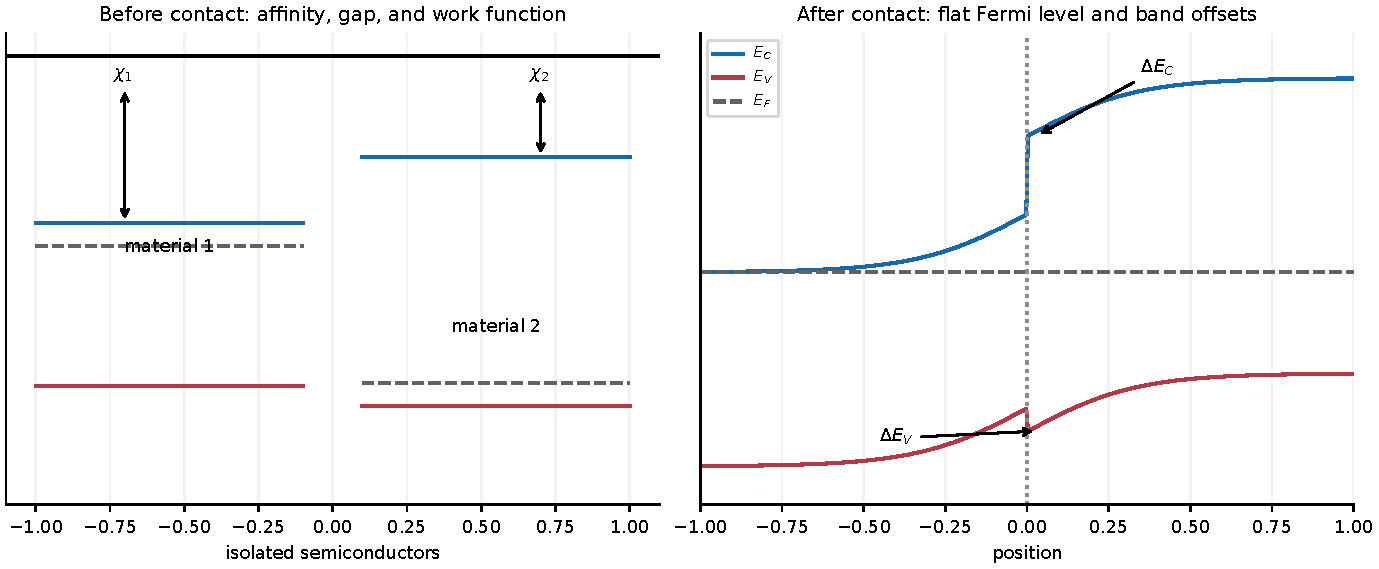
\includegraphics[width=0.94\textwidth]{figures/junction-atlas-heterojunction.pdf}
 \caption{Original isolated-semiconductor and equilibrium heterojunction band
 diagrams showing affinity, gap, work-function difference, a flat equilibrium
 Fermi level, and conduction- and valence-band offsets.  The panels cover the
 subject of Fig.~30 in Sze--Lee Chapter~3 \cite[Sec.~3.7]{szeLee2012}.\figurenotebookmark}
 \label{fig:junction-atlas-heterojunction}
\end{figure}
\figurenotebooktext{figures/20_breakdown-heterojunctions/fig_20_01.ipynb}

\section{Numerical breakdown and lineup checks}

The notebook integrates $A\exp[-B/E(x)]$ on a refined depletion grid and finds
the voltage at which the integral equals one.  It checks quadrature refinement,
monotonicity with voltage, and the expected decrease of breakdown voltage with
background doping.  A separate Anderson-rule calculation verifies the band-gap
identity between the two offsets.

\begin{figure}[htbp]
 \centering
 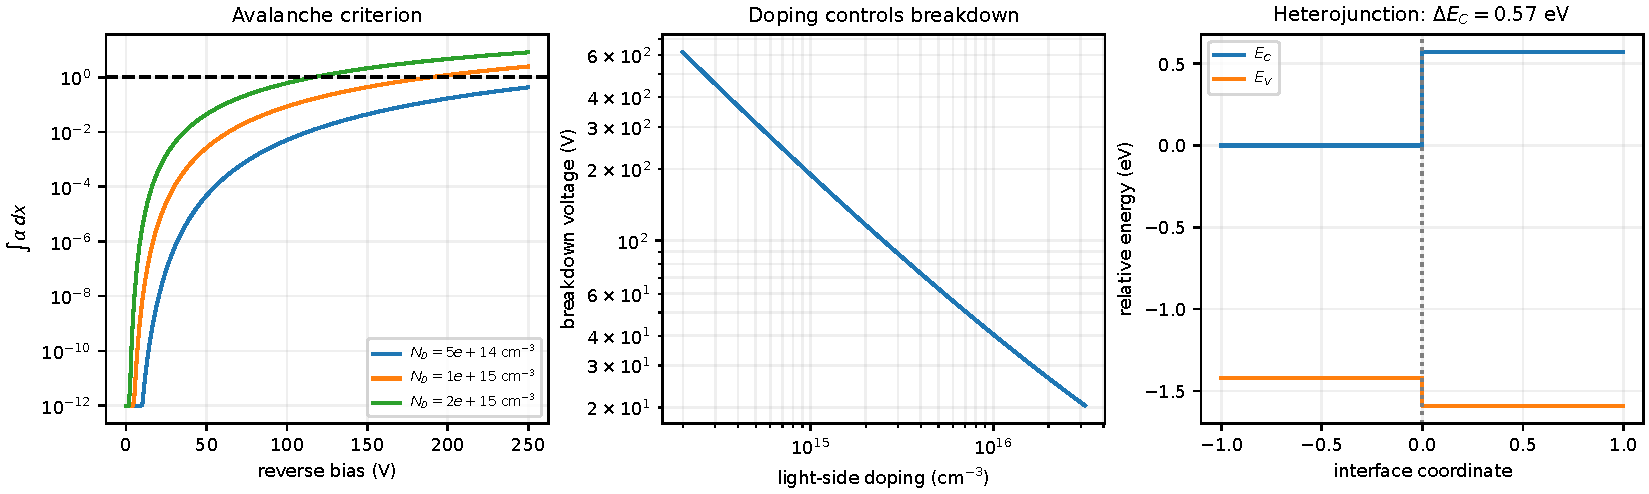
\includegraphics[width=\textwidth]{figures/junction-breakdown-heterojunction.pdf}
 \caption{Avalanche ionization integral, calculated breakdown voltage versus
 lightly doped background concentration, and an ideal electron-affinity-rule
 heterojunction lineup.  The horizontal line marks the equal-coefficient
 avalanche criterion.\figurenotebookmark}
 \label{fig:junction-breakdown-heterojunction}
\end{figure}
\figurenotebooktext{figures/20_breakdown-heterojunctions/fig_20_01.ipynb}

\begin{modelcheck}
The numerical ionization integral is dimensionless and increases monotonically
with reverse voltage.  At the computed root it equals one within the root
solver tolerance.  For the band lineup,
$\Delta E_C-\Delta E_V$ must equal $E_{g2}-E_{g1}$ exactly apart from floating-
point roundoff.
\end{modelcheck}

\begin{boundarybox}
The demonstrated avalanche calculation assumes local ionization, a prescribed
triangular field, and equal electron and hole coefficients.  Dead-space and
nonlocal effects matter when the multiplication region is comparable with the
carrier heating length.  Quantitative heterojunction transport requires
measured offsets, interface charge and recombination, thermionic emission,
tunneling, and possibly quantum confinement.
\end{boundarybox}

\section{Chapter summary}

Tunneling breakdown transfers carriers directly between bands in a narrow,
high-field junction.  Avalanche breakdown is a feedback process driven by
impact ionization across an extended field region.  Geometry can concentrate
field and cause premature breakdown.  Heterojunctions add conduction- and
valence-band discontinuities; electrostatic voltage division and carrier
barriers must then be treated separately.  Numerical quadrature and root
finding turn local ionization data into a junction breakdown prediction.
